%-------------------------------------------------------------------------
% ds-info-S1-boucles-polygones.tex
%-------------------------------------------------------------------------

%-------------------------------------------------------------------------
\documentclass[11pt,a4paper,colorlinks,breaklinks]{article}
%-------------------------------------------------------------------------


%-------------------------------------------------------------------------
%-------------------------------------------------------------------------
% ds-info-S1-preambule.tex
%-------------------------------------------------------------------------

%-------------------------------------------------------------------------
\usepackage{calc}
\usepackage[text={16cm,23cm},centering=true,showframe=false]{geometry}
\usepackage{fancybox,fancyvrb,fancyhdr,lastpage,lineno,import}
\usepackage{longtable,multirow}
\usepackage{xcolor,graphics,xmpmulti,pgf,pgfpages,tikz,wrapfig}
\usepackage{colortbl,color}
\usepackage{amsmath,amssymb,amsfonts}
\usepackage{hyperref,multimedia,rotating,framed,pstricks}
\usepackage{listings,index}
%
%---- pdflatex
%\usepackage[T1]{fontenc}
%\usepackage[utf8]{inputenc}
%---- xelatex
\usepackage{fontspec}
%
\usepackage[french]{minitoc}
\usepackage[french]{babel}
\usepackage[french]{nomencl}
\usepackage[framed,hyperref,standard]{ntheorem}
\usepackage{eurosym,pifont}
%-------------------------------------------------------------------------

%-------------------------------------------------------------------------
\lstset
{
language=Python,
basicstyle=\ttfamily,
identifierstyle=\ttfamily,
keywordstyle=\color{blue}\ttfamily,
commentstyle=\color{gray}\ttfamily,
stringstyle=\color{green}\ttfamily,
showstringspaces=false,
extendedchars=true,
numbers=left, 
numberstyle=\color{blue}\tiny,
frame=lines,
linewidth=0.95\textwidth,
xleftmargin=5mm
} 
%-------------------------------------------------------------------------

%-------------------------------------------------------------------------
\pgfdeclareimage[width=3cm,interpolate=true]{logo-enib}{logo-enib}
%-------------------------------------------------------------------------

%-------------------------------------------------------------------------
\pagestyle{fancy}
\fancyhead{}
\fancyhead[L]{\hspace*{-3em}\begin{minipage}{3cm}\pgfuseimage{logo-enib}\end{minipage}}
\fancyhead[C]{Informatique S1}
\fancyhead[R]{\thepage/\pageref{LastPage}}
\fancyfoot{}
\fancyfoot[L]{}
\fancyfoot[C]{}
\fancyfoot[R]{}
\setlength{\headheight}{80pt}
\setlength{\footskip}{38pt}
\renewcommand{\headrulewidth}{0pt}
\renewcommand{\footrulewidth}{0pt}
%-------------------------------------------------------------------------


%-------------------------------------------------------------------------
\def\entete{\noindent\begin{tabular}{|l|l|l|l|} 
\hline 
 & & & \\ 
\makebox[4.55cm][l]{\bsc{Nom :}} & \makebox[4.5cm][l]{\bsc{Prénom :}} & \makebox[2.5cm][l]{\bsc{Groupe :}} & \makebox[2.75cm][l]{\bsc{Question :}} \\[1mm] 
\hline 
\end{tabular}\\[1mm]
{\footnotesize \textsc{Durée : 15'\hfill Documents, calculettes, téléphones et ordinateurs interdits}}}

\def\notes{\begin{tabular}{|c|c|c|c|}  
\hline 
\makebox[0.5cm]{3} & \makebox[0.5cm]{2} & \makebox[0.5cm]{1} & \makebox[0.5cm]{0} \\  
\hline
\end{tabular}  
} 

\def\autoevaluation{$$\begin{tabular}{|c|c|c|}
\hline
\multicolumn{3}{|c|}{\textbf{Auto-évaluation}} \\
\hline
\textbf{M} & \textbf{V} & \textbf{R} \\
Méthode(s) & Vérification(s) & Résultat(s) \\
\notes & \notes & \notes \\[1mm]
\hline
\end{tabular}$$ $$ $$}

\def\reponse{\mbox{}\hfill \fbox{\huge Réponse page suivante}}
%-------------------------------------------------------------------------

%-------------------------------------------------------------------------
\tikzset{
xmin/.store in=\xmin, xmin/.default=-3, xmin=-3,
xmax/.store in=\xmax, xmax/.default=3,  xmax=3,
ymin/.store in=\ymin, ymin/.default=-3, ymin=-3,
ymax/.store in=\ymax, ymax/.default=3,  ymax=3,
}

\newcommand{\grille}{\draw[color=lightgray] (\xmin,\ymin) grid (\xmax,\ymax);}

\newcommand{\axes}{
	\draw[->] (\xmin,0) -- (\xmax,0);
	\draw[->] (0,\ymin) -- (0,\ymax);
}

\newcommand{\fenetre}{\clip (\xmin,\ymin) rectangle (\xmax,\ymax);}
%-------------------------------------------------------------------------

%-------------------------------------------------------------------------
\def\ga{\textsc{ga}}   
\def\bu{\textsc{bu}} 
\def\zo{\textsc{zo}} 
\def\meu{\textsc{meu}} 
%-------------------------------------------------------------------------


%-------------------------------------------------------------------------
\input{sigle}
%-------------------------------------------------------------------------

\graphicspath{{../../fig/}}



%-------------------------------------------------------------------------

%-------------------------------------------------------------------------
\begin{document}
%-------------------------------------------------------------------------
\entete

\autoevaluation


$$\mbox{\textbf{\large Polygones réguliers}}$$


\paragraph{Questions :} 
En utilisant les instructions de la tortue \logo{}
(module \texttt{turtle}), écrire un algorithme qui dessine un motif géométrique
composé de $(n\times m)$ polygones réguliers alignés sur une grille
ou disposés en quinconce sur la grille.
\vspace*{3mm}

\begin{minipage}[t]{7cm}
\begin{enumerate}
\item décagones (10 côtés) alignés
\item décagones (10 côtés) en quinconce
\item heptadécagones (17 côtés) alignés
\item heptadécagones (17 côtés) en quinconce
\item heptagones (7 côtés) alignés
\item heptagones (7 côtés) en quinconce
\item pentagones (5 côtés) alignés
\item pentagones (5 côtés) en quinconce
\item hendécagones (11 côtés) alignés
\item hendécagones (11 côtés) en quinconce
\item octogones (8 côtés) alignés
\item octogones (8 côtés) en quinconce
\end{enumerate}
\end{minipage}
\hfill
\begin{minipage}[t]{7cm}
\begin{enumerate}\setcounter{enumi}{12}
\item dodécagones (12 côtés) alignés
\item dodécagones (12 côtés) en quinconce
\item hexagones (6 côtés) alignés
\item hexagones (6 côtés)  en quinconce
\item hexadécagones (16 côtés) alignés
\item hexadécagones (16 côtés) en quinconce
\item pentadécagones (15 côtés) alignés
\item pentadécagones (15 côtés) en quinconce
\item tridécagones (13 côtés) alignés
\item tridécagones (13 côtés) en quinconce
\item ennéagones (9 côtés) alignés
\item ennéagones (9 côtés) en quinconce
\end{enumerate}
\end{minipage}
\null\vfill

\centerline{\textbf{Du triangle équilatéral (3 côtés) à l'octadécagone régulier (18 côtés)}}
\centerline{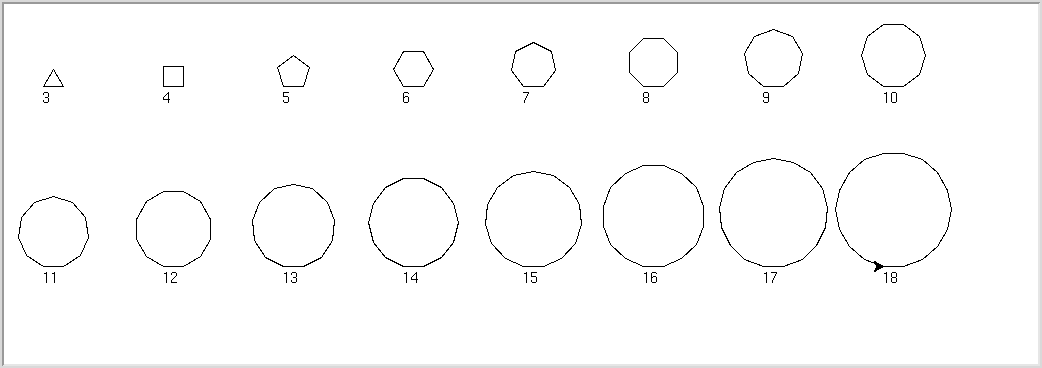
\includegraphics[width=\textwidth]{polygones.png}}


%-------------------------------------------------------------------------
\paragraph{Réponse :}\mbox{}

\noindent\framebox[\textwidth]{$\rule{0cm}{0.96\textheight}$}



%-------------------------------------------------------------------------
\end{document}
%-------------------------------------------------------------------------
